\section[模型]{模型\\Modeling}
In applied works it only rarely happens that the given physical problem is in the exact form

\[ x_{k}=F_{k-1}x_{k-1}+\epsilon_{k} \]

\[ b_{k}=A_{k}x_{k}+e_{k} \]

\begin{figure}[h]
	\centering
	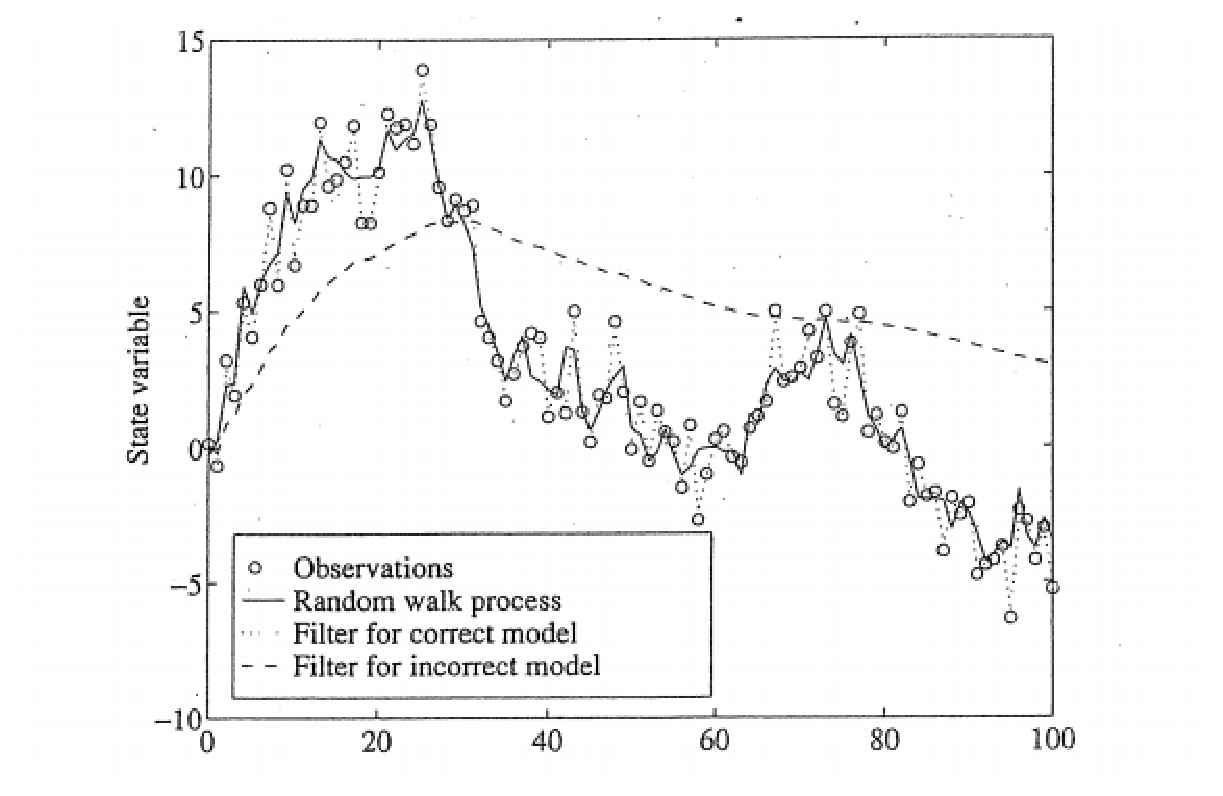
\includegraphics[width=0.7\linewidth]{TeX_files/Part02/chapter05/image/3}
	\caption{Correctly and incorrectly filtered random walk process}
\end{figure}

 
Most often the original problem has to be modified to fit into the appropriate form. This twisting around is often referred to as modeling and it is all-important in Kalman filtering applications. Good modeling leads to good results; bad modeling leads to bad results. It is as simple as that. There are no set rules for the modeling procedure, and it often requires some imagination. Perhaps the best way to become adept at modeling is to look at a wide variety of examples. We start by an example from Brown and Hwang (1997) demonstrating the effects of mis-modeling.
 

\textbf{ Example 5.15} Consider a process that is actually random walk but is incorrectly modeled as a random constant $ c$. We have then for the true model 

\[ x_{k}=x_{k-1}+\epsilon_{k}, \quad \epsilon_{k}=unity Gaussian white noise,\sigma^{2}{x_{0}}=1 \]

\[ b_{k}=x_{k}+e_{k},\quad k=0,1,2,...\sigma^{2}\left\lbrace e_{k}\right\rbrace =0,1\]

and for the incorrect model

\[ x_{k}=c,\quad c~N(0,1) \]
\[ b_{k}=x_{k}+e_{k},\quad k=0,1,2,...\sigma^{2}\left\lbrace e_{k}\right\rbrace=0,1 \]

The wrong model has $ F_{k}=1,\sum\nolimits_{\varepsilon,k}=0,\sum\nolimits_{e,k}=0.1, \hat{x_{0}}=0 $ and $ P_{0}^{-1}=1 $.For the true model the parameters are the same except that $ \sum\nolimits_{\varepsilon,k}=1 $ rather than zero. 

 
 The random walk $x_{0},x_{1},...  $ was simulated using Gaussian random numbers with zero mean and unity variance.The resulting process for 100 seconds is shown in Figure 5.3. A measurement sequence bk of this sample process was also generated using another set of $ N(0, 1) $ random numbers for $ e_{k} $. This measurement sequence was first processed using the incorrect model $ \sum\nolimits_{\varepsilon,k}=0  $ ,and again with the correct model .The results are shown along with the sample process in Figure5.3. In this case the measurement noise is relatively small ($ \sigma\approx0.3 $), and we note that the estimate of the modeled filter does very poorly after the first few steps. This is due to the filter’s gain decreasing with each succeeding step. At the 100th step the gain is more than two orders of magnitude less than at the beginning. Thus the filter becomes very sluggish and will not follow the random walk. Had the simulation been allowed to go further on, it would have become even more sluggish.
 
 The moral to Example 5.15 is simply this. Any model that assumes the process, or any facet of the process, to be absolutely constant forever and ever is a risky model. In the physical world, very few things remain absolutely constant. The obvious remedy for this type of divergence problem is always to insert some process noise into each of the state variables. Do this even at the risk of some degree of suboptimality; it makes for a much safer filter than otherwise. It also helps with potential round off problems. Often a random walk model is a safer model where the time span is large, and it is usually preferred over die truly constant model. 
 
 Choosing an appropriate process model is always an important consideration. A certain amount of common sense judgement is called for in deciding on a model that will fit the situation at hand reasonably well,.but at the same time will not be too complicated. 
 
 For instance no process is a random walk to infinity. At some point it is (band) limited somehow: The troposphere for a short time looks like random walk. But suppose there were no measurements for an entire day? Would our lack of knowledge about the troposphere approach infinity? No, of course not. We know that the troposphere zenith delay can be predicted to be 2.4 meters with about $ 2\textdiscount $ uncertainty or better. So infinity is not the limit. 
 
 \subsection{Computing the Autocorrelation }
 
 It is simple to compute the autocorrelation for an ordered set of data $ a_{0},a_{1}.1_{2},...a_{n-1} $, taken at a constant time interval. First we compute the mean m (the average). Second we may imagine the data arranged in two rows: 
 
 \[ shift = 0:\begin{bmatrix}
 a_{0}&a_{1}&a_{2}&a_{3}&a_{4}&...\\ a_{0}&a_{1}&a_{2}&a_{3}&a_{4}&...
 \end{bmatrix}\quad auto(0)=\sum_{0}^{n-1}a_{i}a_{i}/n \] 
 
 We multiply element $ a_{i}a_{i} $ above each other, and add. Now shift the lower row:
 
 \[ shift = 1:\begin{bmatrix}
 a_{0}&a_{1}&a_{2}&a_{3}&a_{4}&...&\quad\\ \quad&a_{0}&a_{1}&a_{2}&a_{3}&a_{4}&...
 \end{bmatrix}\quad auto(0)=\sum_{1}^{n-1}a_{i}a_{i-1}/n \] 
 
 Again we multiply elements above each other. This time the number of terms is diminished by one. We continue shifting, and each time we divide the sum by the number of data n. The M-file has the following core code: 
 
 \[ auto=autocoor(a) \]
 \[ m=mean(a) \]
 
 \begin{figure}[h]
 	\centering
 	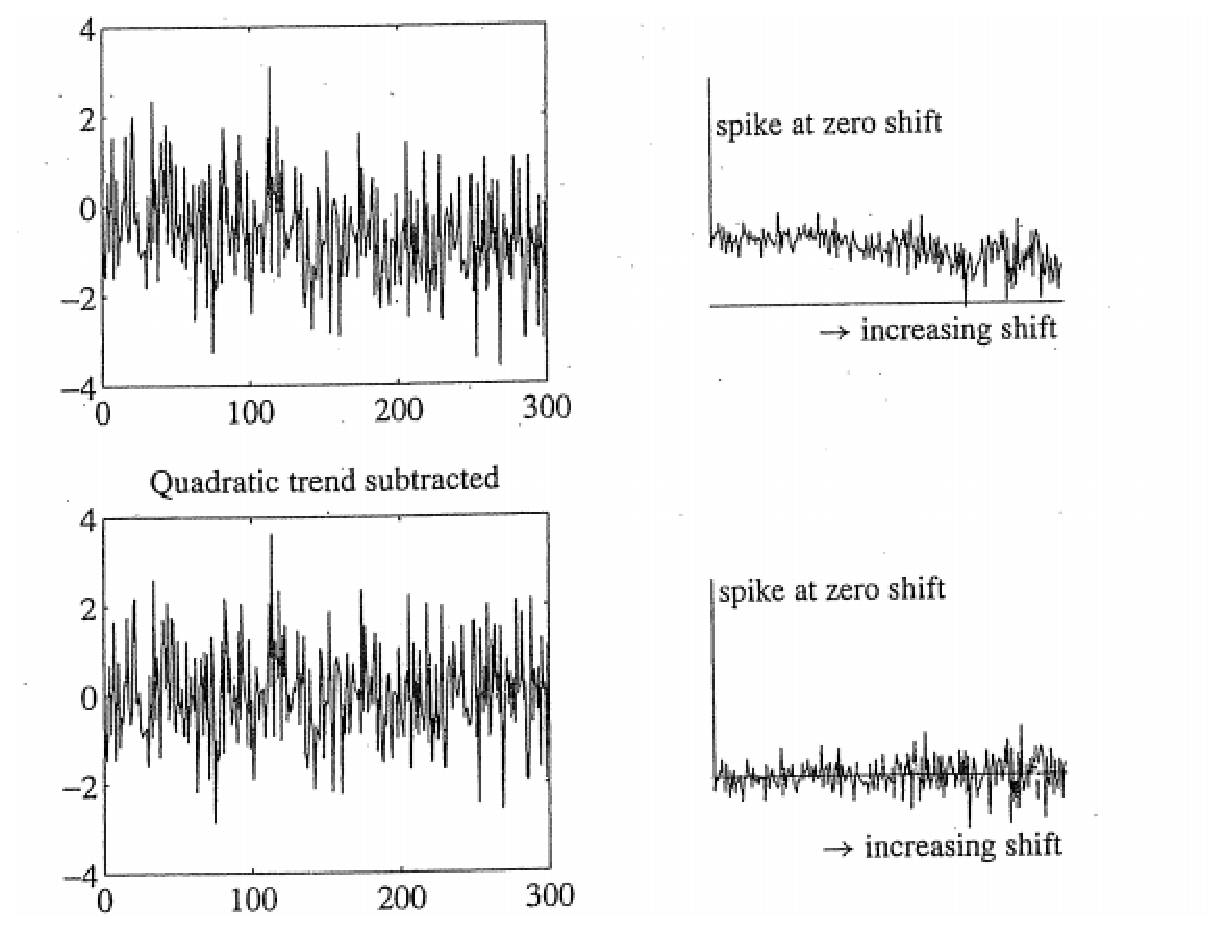
\includegraphics[width=0.7\linewidth]{TeX_files/Part02/chapter05/image/4}
 	\caption{Autocorrelation for random data. The peak at zero measures the variance.}
 	\label{ }
 \end{figure}
 
 
 \[ for \quad shift = 0:n-2 \]
 \[ q=0 ;\]
 \[ for\quad t=1:n-shift \]
 \[ q=q+(a(t)-m)*(a(t+shift)-m); \]
 \[ end \]
 \[ auto(shift+1)=q/n ;\]
 \[ end \]
 
 The sums for large shifts contain only a small number of terms; the overlap count $ n-shift-1 $  is small. It is statistical practice to omit the last  $20/100$(or a similar fraction) of the shifted product sums; they are not so reliable. Luckily enough we are most interested in the autocorrelation for small shifts as those reveal the nature of the data. So the result of autocorr is most important for small shifts,see Figure5.4. 
 
  We divided the sums by$  n $,and not $ n-shift-1 $ .This happens to secure that 
  \begin{equation}\label{5.34}
   R=\begin{bmatrix}
  auto(0)&auto(1)&...&auto(n-1)\\auto(1)&auto(0)&...&auto(n-2)\\ \colon&\colon&\ddots&\colon\\auto(n-1)&auto(n-2)&...&auto(0)
  \end{bmatrix}
  \end{equation}
  
 is positive semi-definite.
 
 
 
 \begin{figure}[h]
 	\centering
 	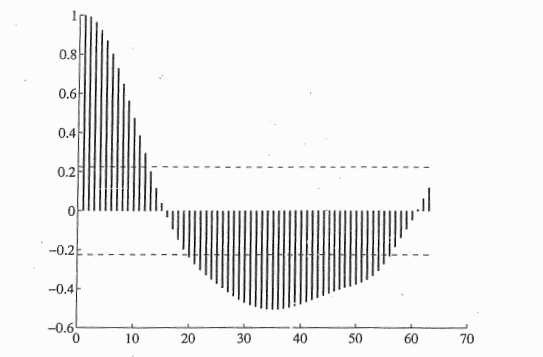
\includegraphics[width=0.7\linewidth]{TeX_files/Part02/chapter05/image/5}
 	\caption{Correlogram for an autocovariance function. The dashed horizontal lines represent the limits $ \pm2/\sqrt{n},n $being 80.}
 	\label{ }
 \end{figure}
  

\subsection{Variance Component Model}

Once again we assume that our observations (signal) are stationary. Furthermore that observations are made at equidistant time invervals.In the following we shall introduce some useful tools for analyzing autocorrelation functions.

 
Often we are furnished with a normalized autocorrelation function. The autocorrelation coefficient $ r_{k} $ is defined as 
\begin{equation}\label{5.35}
r_{k}=\Re_{x}(k)/\Re_{x}(0),\quad k=0,1,...,n-1 
\end{equation}
 

The plot of $ r_{k} $ for varying k is called the correlogram for the random process $ x_{k} $ . One simple use of the correlogram is to check whether there is evidence of any serial dependence in an observed time series. To do this, we use a result due to Bartlett who showed that for a white noise sequence $ a_{k} $ and for large $ n $, $ r_{k}  $ is approximately normally distributed with mean zero and variance $ 1/n $. Thus values of $ r_{k} $  greater than $ 2/\sqrt{n} $ in absolute value can be regarded as significant at about the$  5/100 $ level. If a large number of $ r_{k} $ are computed it is likely that some will exceed this treshold even if ajc is a white noise sequence.

Figure 5.5 shows a correlogram for a receiver clock offsets. The limits $ ± 2/\sqrt{n} $ are exceeded for shift $ 0 $ to $ 12 $ an dalonger sequence from $ k = 20 $ to $  k =56 $.So the correlogram indicates correlation between observations even with shifts up to 56 units of time. 

In practice random processes often show a non-random trend $ \mu_{t} $. With the noise term $ \epsilon_{t} $ we have 

\[ Z_{t}=\mu_{t}+\epsilon{t} \]

We shall demonstrate how to handle this circumstance  by splitting the observation $ Z_{i}(t) $ of the ith series into a starting level $ L_{i}(t) $,a random stationary part $ M_{i}(t) $,and noise $ N_{i}(t) $:
\begin{equation}\label{5.36}
Z_{t}(t_{k})=L_{i}(t_{0})+M_{i}(t_{k})+N_{i}(t_{k})
\end{equation}
 

All observations for all experimental subjects$  i = 1, 2, ...,   m $ are taken at equidistant times $ t_{0},t_{1},...t_{k},L_{i} $.is defined at time $ t_{0} $ while the random variables depend on time $ t_{k} $ . $ L_{i} $ is independent of $ L_{j} $ for $ i\neq j $and is distributed as $ N(0,\lambda^{2}) $ . The noise $ N_{i}(t_{k}) $ is distributed as $ N(0,\nu^{2}) $ and independent in time as well as between subjects. Finally $ M_{i}(t_{k}) $ is distributed as $ N(0,\mu^{2}) $  and independent between subjects and with $ R(k)=\mu^{2}r(k) $ .  We remember that $ r(0) = 1 $ and $ r(k)\rightarrow 0 $ for $ k\rightarrow \infty $. The three components $  L_{i},M_{i}, $ and $ N_{i} $ are assumed mutually independent.Hence the observational variance is 

\[ R_{Z}(0)=Var(Z_{i}=\lambda^{2}+\mu^{2}+\nu^{2}) \]

The covariance between $ Z_{i}(t_{l}) $ and $ Z_{j}(t_{m}) $ is
\begin{equation*}
\begin{aligned}
\sigma (Z_{i}(t_{i}), Z_{j}(t_{m}))&=E\left\lbrace Z_{i}(t_{i}) Z_{j}(t_{m})\right\rbrace\\
&=E\left\lbrace(L_{i}(t_{0})+M_{i}(t_{l})+N_{i}(t_{l}))(L_{j}(t_{0})+M_{j}(t_{m})+N_{j}(t_{m}))  \right\rbrace\\
&= E\left\lbrace L_{i}L_{j}\right\rbrace +E\left\lbrace M_{i}(t_{l})M_{j}(t_{m}) \right\rbrace =(Var(L_{i})+\mu^{2}r_{Z}(t_{m}-t_{l}))\delta_{ij}
\end{aligned}
\end{equation*}
\[ (\lambda^{2}+\mu^{2}r_{Z}(k))\delta_{ij} \]

Note that especially for $ i\neq j $ the covariance is zero due to the independence of subjects. 

For a moment we dwell on the autocorrelation $ R_{Z}{k} $.The observational error $ N_{i}(t_{k}) $is not equal to zero; this implies that $ R_{Z}(k) $ does not approach $ R_{Z}(0) $ for $ k\rightarrow 0 $ .Also $ R_{Z}(k) $ does not approach 0 for $ k\rightarrow \infty $. This is caused by the subject specific random variable $ L_{i} $ .

 From (5.34) we remember R and let E denote a matrix with all ones, then the covariance matrix can be written as  
 
 \[ \sum = \lambda^{2}E+\mu^{2}R+\nu^{2}I \]
 
 Now we are ready to introduce the variogram function 
 \begin{equation}\label{5.37}
 V(k) = 1/2E\left\lbrace (Z_{i}(t_{l})-Z_{i}(t_{m}))^{2} \right\rbrace
 \end{equation}
  
 
 we have 
 
 \[ Z_{i}(t_{l})-Z_{i}(t_{m})=M_{i}(t_{l})-M_{i}(t_{m})+N_{i}(t_{i})-N_{i}(t_{m})\]
 
 and remembering that $ M_{i} $ and $ N_{i} $ are independent we get
 \begin{equation*}
 \begin{aligned}
 V(k)&=1/2E\left\lbrace (M_{i}(t_{l})-M_{i}(t_{m}))^{2}\right\rbrace+1/2E\left\lbrace (N_{i}(t_{l})-N_{i}(t_{m}))^{2}\right\rbrace\\
 &=\mu^{2}(1-r_{Z}(k))+\nu^{2} 
 \end{aligned}
 \end{equation*}
  
 
   Figure 5.6 shows a variogram with the three variance components $ \lambda^{2} ,u^{2}$ and $ \mu^{2} $. Remember $ r_{Z}(0)=1 $  and hence $ lim_{k\rightarrow 0}V(k)=\nu^{2} $ .We can read $ \nu^{2} $ from the figure as the intercept with the ordinate axis.
 
  For any stationary, random process we have $ r_{Z}(k)\rightarrow 0 $ for $ k\rightarrow 0 $. Thus $ V(\infty)=\mu^{2}+\nu^{2} $ . So the variance $\mu^{2} $ within the individual subjects is found as $ V(\infty) $ minus $ \mu^{2} $ .
 
 
 \begin{figure}[h]
 	\centering
 	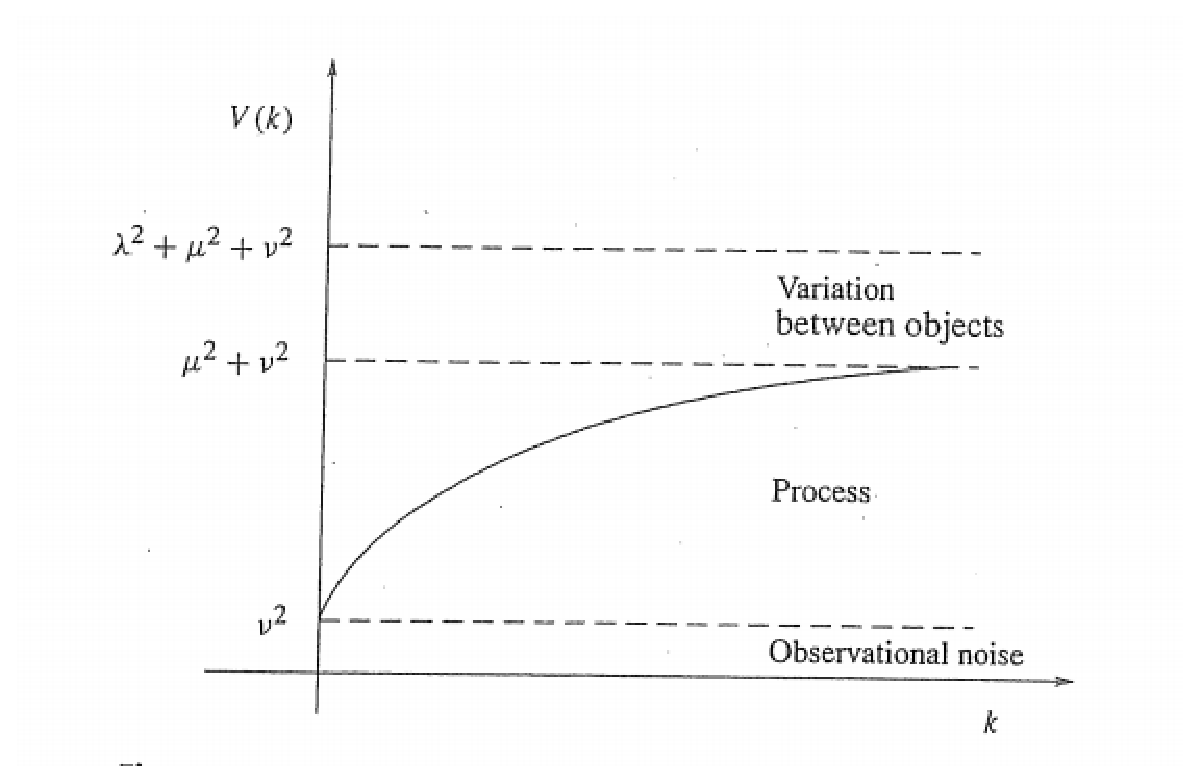
\includegraphics[width=0.7\linewidth]{TeX_files/Part02/chapter05/image/10}
 	\caption{Variogram illustrating the three variance components}
 	\label{ }
 \end{figure}
 
 
 The total variance for all observations $ Z_{i} $ is estimated by taking data across experimental subjects. Again under the assumption of mutually independent processes the total varianceis computed as the mean value of $ (Z_{i}(t_{l})-Z_{j}(t_{m}))^{2}/2 $ for all / and m and all$  i $ and $ j $ with $ i\neq j $.This makes $ M=\sum\nolimits_{i}(_{2}^{n_{i}}) $ terms, where $ n_{i} $ is the number of observations in the $ i $ th series: 
 
 \[ \lambda^{2}+\mu^{2}+\nu^{2}=1/2M \sum_{i\neq j}(Z_{i}(t_{l})-Z_{j}(t_{m}))^{2} \]
 
 The total variance also is illustrated in Figure 5.6. The variance $ \lambda^{2} $ for the population can be read at the ordinate axis, too.
 
 Two common examples of autocorrelation functions are the exponential correlation function
 \begin{equation}\label{5.38}
  r(k)=e^{-\alpha k}
 \end{equation}
  
 
 and the Gaussian correlation function
 \begin{equation}\label{5.39}
  r(k)=e^{-\alpha k^{2}}
 \end{equation}
 
 
 In Figure 5.7 we have sketched the autocorrelation function for (5.38) and (5.39) and the corresponding variograms. The exponential correlation function decreases strongly for small time differences k while the Gaussian correlation function has a strong correlation overa larger time. Later it decreases rapidly. 
 
 Example 5.16 For a demonstration of the theory we use one-way differences between a receiver and a satellite. We use satellites with pseudo random noise (PRN) codes 2, 9,16, 23, 26, and 27. We concentrate on ionospheric delays for epoch k. We observe on two frequencies to cancel the main error in the delay $ I_{k} $:
 
 \[ I_{k} =\frac{(\Phi_{2,k}-\lambda_{2}N_{2})-(\Phi_{1,k}-\lambda_{1}N_{1})}{1-(f_{1}/f_{2})^{2}} \]
 
 \begin{figure}[h]
 	\centering
 	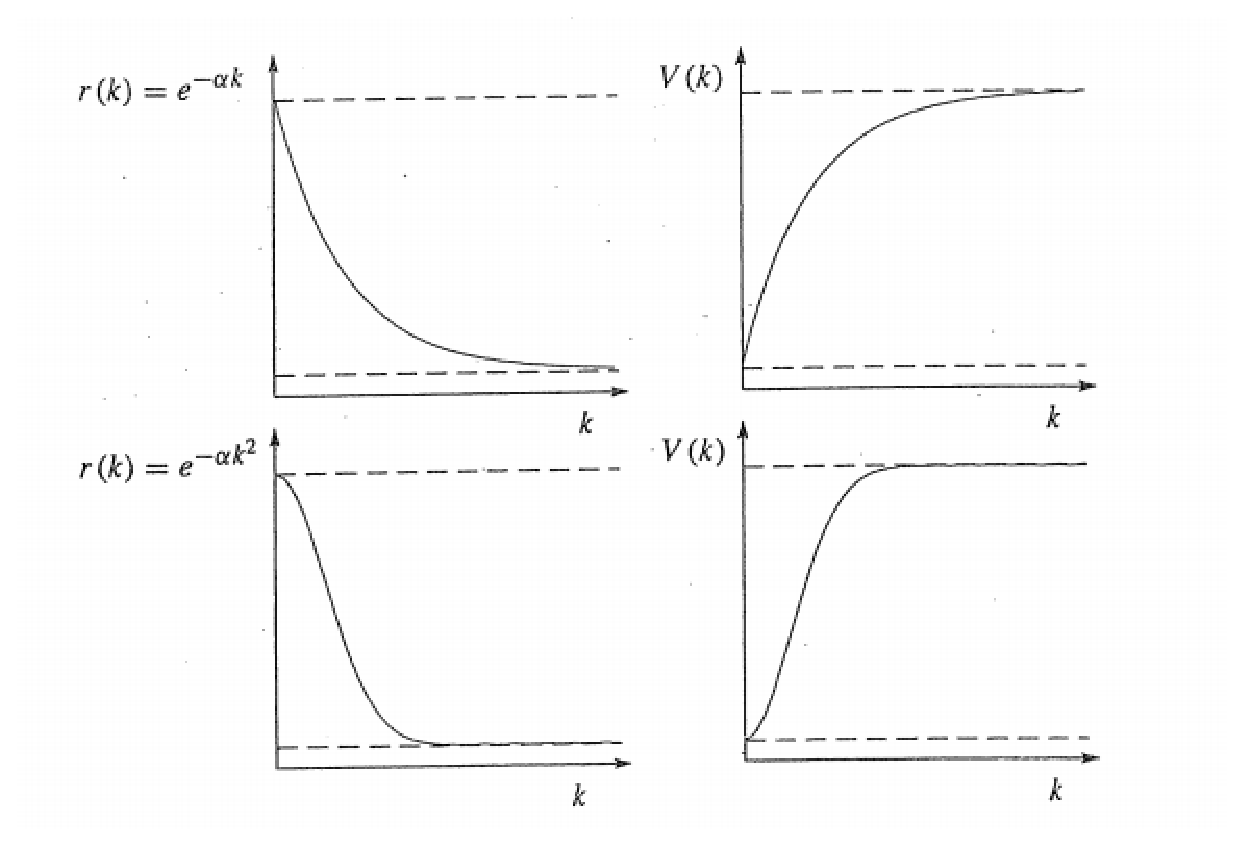
\includegraphics[width=0.7\linewidth]{TeX_files/Part02/chapter05/image/6}
 	\caption{Exponential and Gaussian autocorrelationfunctions and variograms}
 	\label{ }
 \end{figure}
 
 
 Figure 5.8 depicts $ I_{k}$ as calculated for one-ways, their differences and their differences again which are the so-called double differences. The actual baseline length is 4.6 km. For one-ways $ I_{k} $ typically varies from 5-15m. Single differences have $ I_{k} $ values of 2.5-3m and double differences between $ -0.2-0.2 $ m. Note that the mean values of elevation angle for the individual PRN’s are listed in Table 5.3. From this you observe that $ I_{k} $ depends strongly on the elevation angle for the single PRN. 
 
 Now we turn to autocorrelation functions for $ I_{k} $.To eliminate a possible trend in an observation series one often starts the investigations from differences in time:$ I_{K}-I_{K-1} $. The autocorrelation for the differenced ionospheric delay for the one-way to PRN 2 is shown in Figure 5.9 (upper left). The spike at zero equals the variance of a difference $ I_{K}-I_{K-1} $. Next we compute the autocorrelation for the undifferenced $ I_{k} $. The result is
 
 \[\textbf{ Table 5.3} Autocorrelation of ionospheredelay for one-ways \] 
 \[ \begin{tabular}{lccc}
 \hline
 $ \quad$ & $ Elevation  $ & $\sigma_{1}(m)$&$Shift for firstzero  $ \\
 \cline{1-4}
  $ PRN$ & $ (^{\circ}) $ & $ master \quad rover $&$master \quad rover  $ \\
   $ 26$ & $ 68.9 $ & $ 0.08 \quad0.11 $&$35\quad 30  $ \\
  $ 2$ & $ 59.0 $ & $ 0.08 \quad0.04 $&$15\quad 35  $ \\
  $ 27$ & $ 28.0 $ & $ 0.39 \quad0.35 $&$30\quad 32  $ \\
  $ 16$ & $ 22.8 $ & $ 0.77 \quad0.71 $&$30\quad 30  $ \\
  $ 23$ & $ 20.4 $ & $ 0.17 \quad0.19 $&$12\quad 20  $ \\
  $ 9$ & $ 18.5 $ & $ 0.48 \quad0.19 $&$15\quad 30  $ \\
  
 \hline
 \end{tabular} \] 
      	  
  \begin{figure}[h]
  	\centering
  	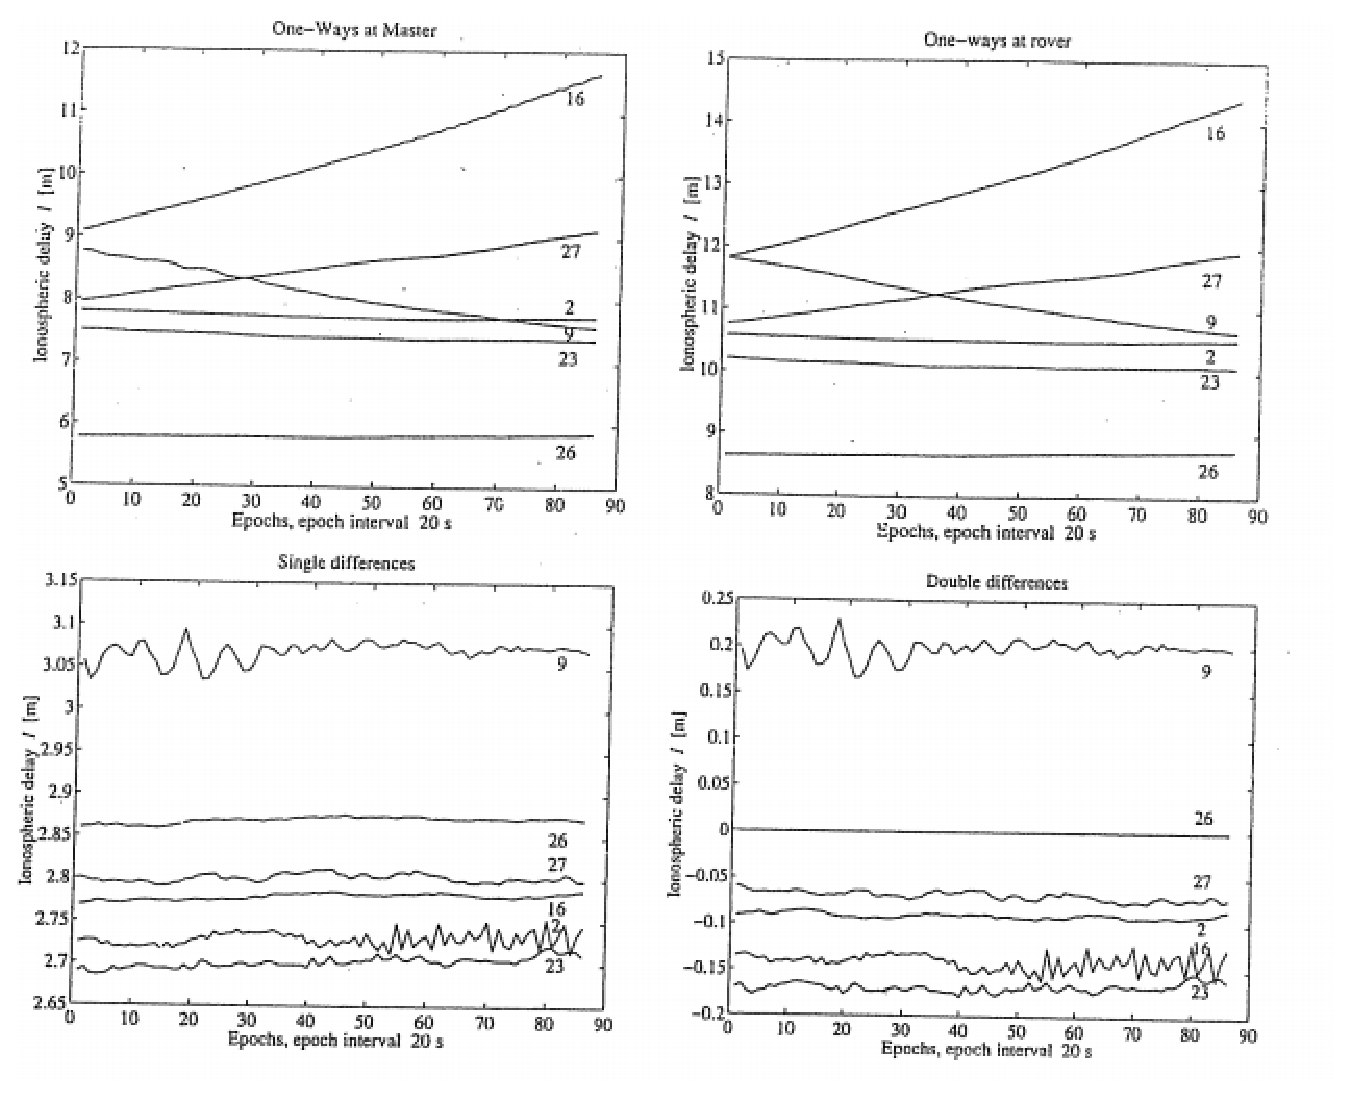
\includegraphics[width=0.7\linewidth]{TeX_files/Part02/chapter05/image/7}
  	\caption{Exponential and Gaussian autocorrelationfunctions and variograms}
  	\label{}
  \end{figure}
  
 shown at the upper right. This evidently reflects a remaining systematic term in the delay . Our ultimate goal is to model this part and subsequently subtract it from the actual delay, hopefully leaving only white or nearly white noise. Knowing a good model we can with a high degree of accuracy predict the ionospheric delay in time $ \delta_{t} $ and also with distance $ d $. 
  
 We continue computing the autocorrelation for $ I_{k} $ for a single difference. When computing autocorrelation for differences we must remember the rules given in (5.13). This implies that we have to compute cross correlations. The lower left of Figure 5.8 shows the result for PRN 2. 
 
 In Table 5.3 we have $ \sigma_{1}=2 $cm for PRN 2 and $ \sigma_{1}=77 $cm for PRN 16. The numbers in Table 5.3 are produced by calls like 
 
 \[ one_way(m)(27)\quad and \quad autocorr(x(2,:)^{'}) \]
 
 However these numbers diminish to 4 mm and 9 mm for single differences and 2 mm and 9 mm for double differences. The general M-file for this example is called $ oneway_{i} $.
 
 Because of varying geometry, $ I_{k} $ will vary with different baseline lengths $  d = 5, 25, 50, 100,500, 1000 $ km, say. So we suggest the interested reader to explore this sort of investigation with the final goal of determining the variance of differential ionosphere $ \sigma_{0}^{2} $ , correlation time $  T  $, and correlation length $ D $ 。
 
 \begin{figure}[h]
 	\centering
 	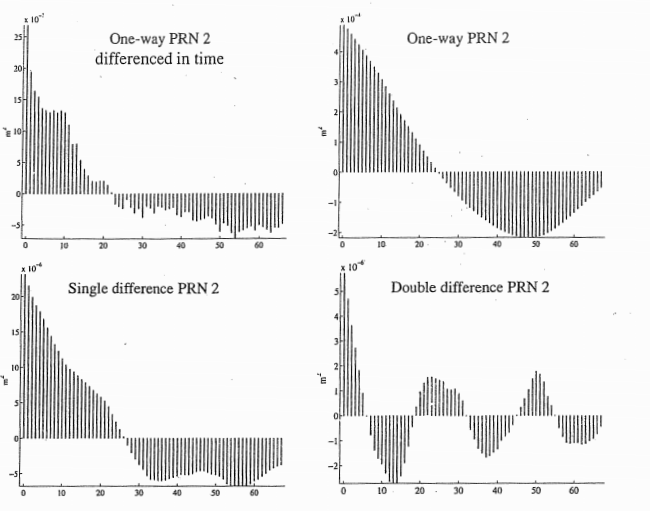
\includegraphics[width=0.7\linewidth]{TeX_files/Part02/chapter05/image/8}
 	\caption{Autocorrelation fo rionospheric delay to PRN 2}
 	\label{ }
 \end{figure}
 
 
  Upper left shows difference in time:$ I_{k}-I_{k-1} $ ,upper right the one-way, lower left the single difference, and lower left the double difference.Note the various orders of magnitude.sample interval $ \delta_{t} $ and baseline length $ d $:
 \begin{equation}\label{5.40}
  R_{x}(k,d)=\sigma_{0}^{2}e^{-|\delta_{t}|/T} e^{-d/D}
 \end{equation}
  
 
 This function $ R_{x} $ has been determined from double differenced phase observations in Goad and Yang (1994). The authors assume staiionarity and an exponentially correlated process: they estimated $ T $ to 64 min., $ \sigma_{0}^{2}=2m^{2} $, and D $ \approx $ 1500km. In general you may adjust a Gauss-Markov process to the paramete $ \sigma^{2} $ and $ \alpha $.At $ k = 0 $ we fit $ \sigma_{0}^{2} $,and at the 1/e-point we fit $ \alpha $. 
 
 It is known that the ionospheric delay has a distinct daily variation. In Klobuchar (1996) we find an approximate expression for $ I $ in meters as function of local time $  t $ in hours: 
 
 \[ I=2.1+0.75\cos((t-14)2\pi/28) \]
 
 This value is valid in the direction of zenith. To get the increased value of $ I $ in a direction with elevation angle $ El $ in half circles (the range of $ El $ is 0-0.5, half circle times $ \pi $ equals radians) we have to multiply by the obliquity factor
 
 \[ F(El)=1+16(0.53-El)^{3} \]
 
 \begin{figure}[h]
 	\centering
 	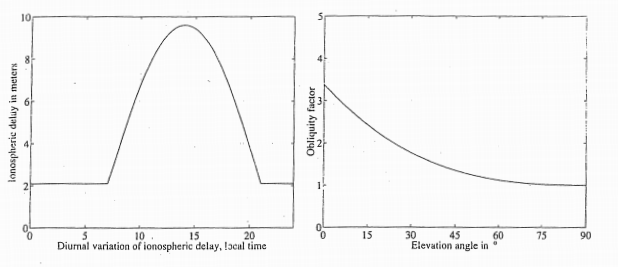
\includegraphics[width=0.7\linewidth]{TeX_files/Part02/chapter05/image/9}
 	\caption{Ionospheric delay model as function of local time and elevation angle}
 	\label{ }
 \end{figure}
 
 
 This expression is based on a formula given in IS-GPS-200 (2007). Figure 5.10 shows the graphs of $ I $ and $ F(El) $. The small constant level of delay equal to 2.1m represents the delay at night. As the sun rises and sets, the ionospheric model gives rise to the cosineTaspsd pulsefor daytime. 
 
When interpreting an autocorrelation function it is useful to remember the following important properties:

 Maximum value Theautocorrelation function has a maximum at zero shift:  
 
 \[ E\left\lbrace x^{2}(t)\right\rbrace  = R_{x}(k) \]
 
 Symmetry conditions The autocorrelation function is an even function 
 
 \[ R_{x}(k) = R_{x}(-k) \]
 
 while the cross correlation satisfies 
 
 \[ R_{xy}(k)=R_{yx}(-k) \]
 
 Mean-square value The cross correlation is bounded by
 
 \[ |R_{xy}(k)|^{2}\leq R_{x}(0)R_{y}(0)\leq\frac{1}{2}((R_{x}(0))^{2}+(R_{y}(0))^{2}) \]
 
 Periodic component The autocorrelation has a periodic component if $  x $ has one.
 
  \textbf{Remark 5.1} (Filter theoretical interpretation of the technique of differencing) We may look at double differenced data $ D $ as made up of two single difference measurements $ S_{i} $: $ D=S_{1}-S_{2} $.Each of these is made up simplistically as $ S_{i}=\rho_{i}+t $ where $ \rho_{i} $ is pseudorange and $ t $ is receiver clock offset converted to length by multiplication by $ c $..Note that $ t $ is the same in both. So double differencing doesremove rhis clock error. 
  
  We illustrate a few basic facts about differencing.Start with two single differences: 
  
  \[ S_{1}=\rho_{1}+t \]
  \[ S_{2}=\rho_{2}+t \]
  
  and their double difference:
  
  \[ S_{2}-S_{1}=\rho_{2}-\rho_{1} \]
  
  For the double difference the situation has changed. We have one less equation and cannot estimate $ t $.You could estimate from single differences but the a priori clock variance $ \sigma_{clock}^{2} $ must be infinite; otherwise you introduce a third measurement, which you do not have in the double difference case. So one case has $ S_{1} $, $ S_{2} $, and $ \sigma_{clock}^{2} $. This is equivalent to $ S_{1} $, $ D $, and  $ \sigma_{clock}^{2} $. If  $ \sigma_{clock}^{2} = \infty $ it really means it is of no value. So this is equivalent to $ S_{1} $ and $ D $. Now since the double differences do not involve the clock explicitly, the only use to be made of $ S_{1} $ is to estimate the clock. Since a clock estimate is not needed by double differencing, $ D $ stands by itself in estimating position. 
  
  However if $ \sigma_{clock}^{2}<\infty $ then this couples all three measurements in which case all three should be processed together. It does not matter whether $S_{1},S_{2},t  $ or $ S_{1},D,t $ or $ S_{2},D,t $ is used. If you treat clocks as having infinite variance at each epoch and then plot their estimates, you will see that clocks do not drift with infinite variance. So theoretically it is correct that we do know something about clock drift, and using double differences alone does not allow us to take advantage of this knowledge (because t cancels). 
  
  Now the difficult question is “ to what degree do receiver clocks drift randomly?” Clearly different receivers have vastly differing (usually quartz) clocks. The best opportunity would be for the International GPS Service for Geodynamics (IGS) to drive their receivers used for orbit calculations with rubidium or,even better,cesium oscillators. Even betteryet would be hydrogen masers, but presently they are just too expensive to consider. Then a more descriptive random model with smaller variances could prove useful. Quartz clocks drift so wildly relative to centimeter positioning requirements, that trying to model them would add little to improving positions.So we may conclude:
  
  
   - Double differencescan be conceived as a filter where the clock behavior is modeled as white noise with infinite variances. 
   
   - Using single differences with analytical prediction of receiver clock offset is better than using double differences if the variances in the prediction is less than infinity,
 
 \subsection{Aspects of Random Processes }
 
  We have presented three basic models: random walk, random ramp, and an exponentially correlated process. Each one introduces a special pattern for how random errors interact. If the model is chosen correctly the residuals should be white, noise. A good measure for the randomness of errors is to look at their autocorrelation. Or in other words: A given autocorrelation function is based on a given model. If the model fits the data, the error autocorrelation function ideally is white noise.
  
   Pure observational errors will show a very clear spike at zero. Systematic errors will give an autocorrelation that remains large, even far away from zero. To demonstrate the autocorrelation for random data we call the M-file $ model_g $(randn(1,300)). The result was shown in Figure 5.4. Here we have an autocorrelation function which has a spike at zero. This spike is a measure for the variance of observation. The global features of the autocorrelation function (away from shift = 0) originate from the model. If the autocorrelation drops off significantly at a certain distance from zero we speak of a band limited process. 
   
   Sometimes we are lucky to know the physics behind a problem. Then it is often given in terms of a differential equation. 
   
   Example 5.17 We describe a procedure starting from a differential equation, leading to the discrete state equation. The z-transform exhibits poles of the solution and these poles determine whether the filter is stable or not.
   
   The actual differential equation describes a forced motion for a body with mass $ m $, damping constant $ d $,and spring modulus $ c $, all under the influenceof an external force $ f $: 
   \begin{equation}\label{5.41}
    m \ddot x + d \dot{x} +cx = f
   \end{equation}
   
   
   The actual displacement of the body is $ x(t)=\int \ddot{x}(t)dt  $ and we differentiate to get $ x_{k}\approx x_{k-1}+\dot{x}_{k-1} $ with $ \delta_{t}=1 $. Furthermore
   \begin{equation}\label{5.42}
   \dot{x}(t)=\int \ddot{x} (t)dt \quad and \quad \dot{x}_{k}\approx\dot{x}_{k-1}+\ddot{x}_{k-1}
   \end{equation}
   
   
   The discrete form of equation (5.41)is
   
   \begin{equation}\label{5.43}
   \ddot{x}_{k-1}=- \frac{d}{m}\dot{x}_{k-1}-\frac{c}{m}x_{k-1}+\frac{f}{m}
   \end{equation}
   
   
   Insertion of (5.43) into (5.42) yields
   
   \[ \dot{x}_{k}=\dot{x}_{k-1}+(- \frac{d}{m}\dot{x}_{k-1}-\frac{c}{m}x_{k-1}+\frac{f}{m}) \]
   
   Hence in matrix form the state equation become
   
   \[ \begin{bmatrix}
   x_{k}\\\dot{x}_{k}
   \end{bmatrix} = \begin{bmatrix}
   1&1\\-c/m&1-d/m
   \end{bmatrix} \begin{bmatrix}
   x_{k-1}\\\dot{x}_{k-1}
   \end{bmatrix}+\begin{bmatrix}
   0\\f/m
   \end{bmatrix}\]
   
   
   Random walk is the special case with $ c = 0 $ and $ d = 0 $. There is no spring force and no damping:
   \begin{equation}\label{5.44}
   \begin{bmatrix}
   x_{k}\\\dot{x}_{k}
   \end{bmatrix} = \begin{bmatrix}
   1&1\\0&1
   \end{bmatrix} \begin{bmatrix}
   x_{k-1}\\\dot{x}_{k-1}
   \end{bmatrix}+\begin{bmatrix}
   0\\f/m
   \end{bmatrix} 
   \end{equation}
    
   
   We substitute the state variables by $ X_{1,k}=x_{k},X_{2,k}=\dot{x}_{k},F(z)=f/m $:
   \begin{equation}\label{5.45}
   \begin{bmatrix}
   X_{1,k}\\X_{2,k}
   \end{bmatrix} = \begin{bmatrix}
   1&1\\-c/m&1-d/m
   \end{bmatrix} \begin{bmatrix}
   X_{1,k-1}\\X_{2,k-1}
   \end{bmatrix}+\begin{bmatrix}
   0\\F(z)
   \end{bmatrix} 
   \end{equation}
    
   
   The displacement of the body from static equilibrium is $ X_{1,k} $ and $ X_{2,k} $ is the instantaneous velocity of the body.
   
   The solution of this discrete system is found via z-transforms $ X_{1}(z)=\sum X_{1,kz^{-k}} $ and $ X_{2}(z)=\sum X_{2,kz^{-k}} $.The transform of (5.45) is
   
   \[ zX_{1}(z)=X_{1}(z)+X_{2}(z) \]
   
   \[ zX_{2}(z)=-\frac{c}{m}X_{1}(z)+(1-\frac{d}{m})X_{2}(z)+F(z) \]
   
   We rewrite the lastequation as 
   
   \[ X_{2}(z)(z-(1-\frac{d}{m}))=- \frac{c}{m} X_{1}(z)+F(z) \]
   
   Then insertion of $ X2(z) $ into the first equation gives 
   
   \[ zX_{1}(z)=X_{1}(z)+\frac{-(c/m)X_{1}(z)+F(z)}{z-(1-d/m)} \]
   
   or
   
   \[ (z^{2}-(2-\frac{d}{m})z+(1-\frac{d}{m}+\frac{c}{m}))X_{1}(z)=F(z) \]
   
   The position $ X_{1}(z) $ of the body is given by
   
   \[ \frac{X_{1}(z)}{F(z)}=\frac{1}{z^{2}-(2-d/m)z+(1-d/m+c/m)} \]
   
   The random walk case with $ c=0 $ and $ d=0 $ gives
   
   \[ \frac{X_{1}(z)}{F(z)}=\frac{1}{z^{2}-2z+1}=\frac{1}{z-1}\frac{1}{z-1} \]
   
   The function $ X_{1}(z) $ has a multiple pole at $ z =1 $. In general if all poles are within the unit circle we deal with a stable filter. If one or more poles are outside the unit circle we have an unstable filter.The present case with $ z = 1 $ is most delicate. The neighborhood of $ z =1 $ is a true “minefield”  .
   
   The z-transform of the impulse response is the transfer function $ H (z) $. Input and output are connected by $ H (z) $ and it is the key to an optimal control. This leads further to explicitexpressionsforautocorrelationandpowerspectraldensity. However,thisrelatively simple example is at the limit of complexityfor finding closed form solutions to algebraic equations by purely algebraic means. So we do not want to present more theory, because in most real world examples numbers rather than formulashave to describe reality.
   
   \textbf{Example 5.18} We want to combine a random walk and white noise in the dynamic linear model 
   
   System equation :$ x_{k}=x_{k-1}+\epsilon_{k},\epsilon_{k}~N_{1}(0,\sigma_{\epsilon}^{2})$
   Observation equation:$ b_{k}=x_{k}+e_{k},e_{k}~N_{1}(0,\sigma_{e}^{2}) $
   
   This is the simplest possible model which has a surprisingly wide range of applications.
   
   We summarize this chapter by repeating the essential pointsfor a Gauss-Markov process: 
   
   Autocorrelation $ \Re_{x}(k)=\sigma^{2}e^{-\alpha|k|} $
   Process $ x_{k}=e^{-\alpha|\delta_{t}|}x_{k-1}+\epsilon_{k} $
   
   Variance $ \sigma_{\epsilon_{k}}^{2}=E\left\lbrace \epsilon_{k}^{2} \right\rbrace =\sigma^{2}(1-e^{-2\alpha|\delta_{t}|})$  to be used on the diagonal of the filter covariance matrix $ \sum\nolimits_{\epsilon,k} $ ,see Chapter 8!
   	